\chapter{Data Generation}\label{Ch:datagen}

Automating artifact detection requires large amounts of data (i.e. corrupted frames), which is extremely limited. Therefore, it was critical that we generate our own data that will well represent the actual distribution of corrupted images. The prototype for our ``synthetic'' data was a sample of about 20 images provided by AMD that were claimed to be representative of artifacts seen most frequently (see Figure \ref{fig:bugs}). The \texttt{Glitchify} software was then produced to artificially create images with different types of corruptions seen in the sample set. Unlike artifacts shown in Figure \ref{fig:bugs}, some of the images in the sample appeared to have highly content-related artifacts, which would be infeasible to reproduce without using laborious segmentation methods. For example, the leftmost image in Figure \ref{fig:hard} exhibits a warrior with a missing corpus, however, some elements of his armor are displayed. The other picture in Figure \ref{fig:hard} contains a car with missing color textures. Since recreating such artifacts would have required object recognition techniques, this study did not address such content-related corruptions.

\begin{figure}[H]
\centering
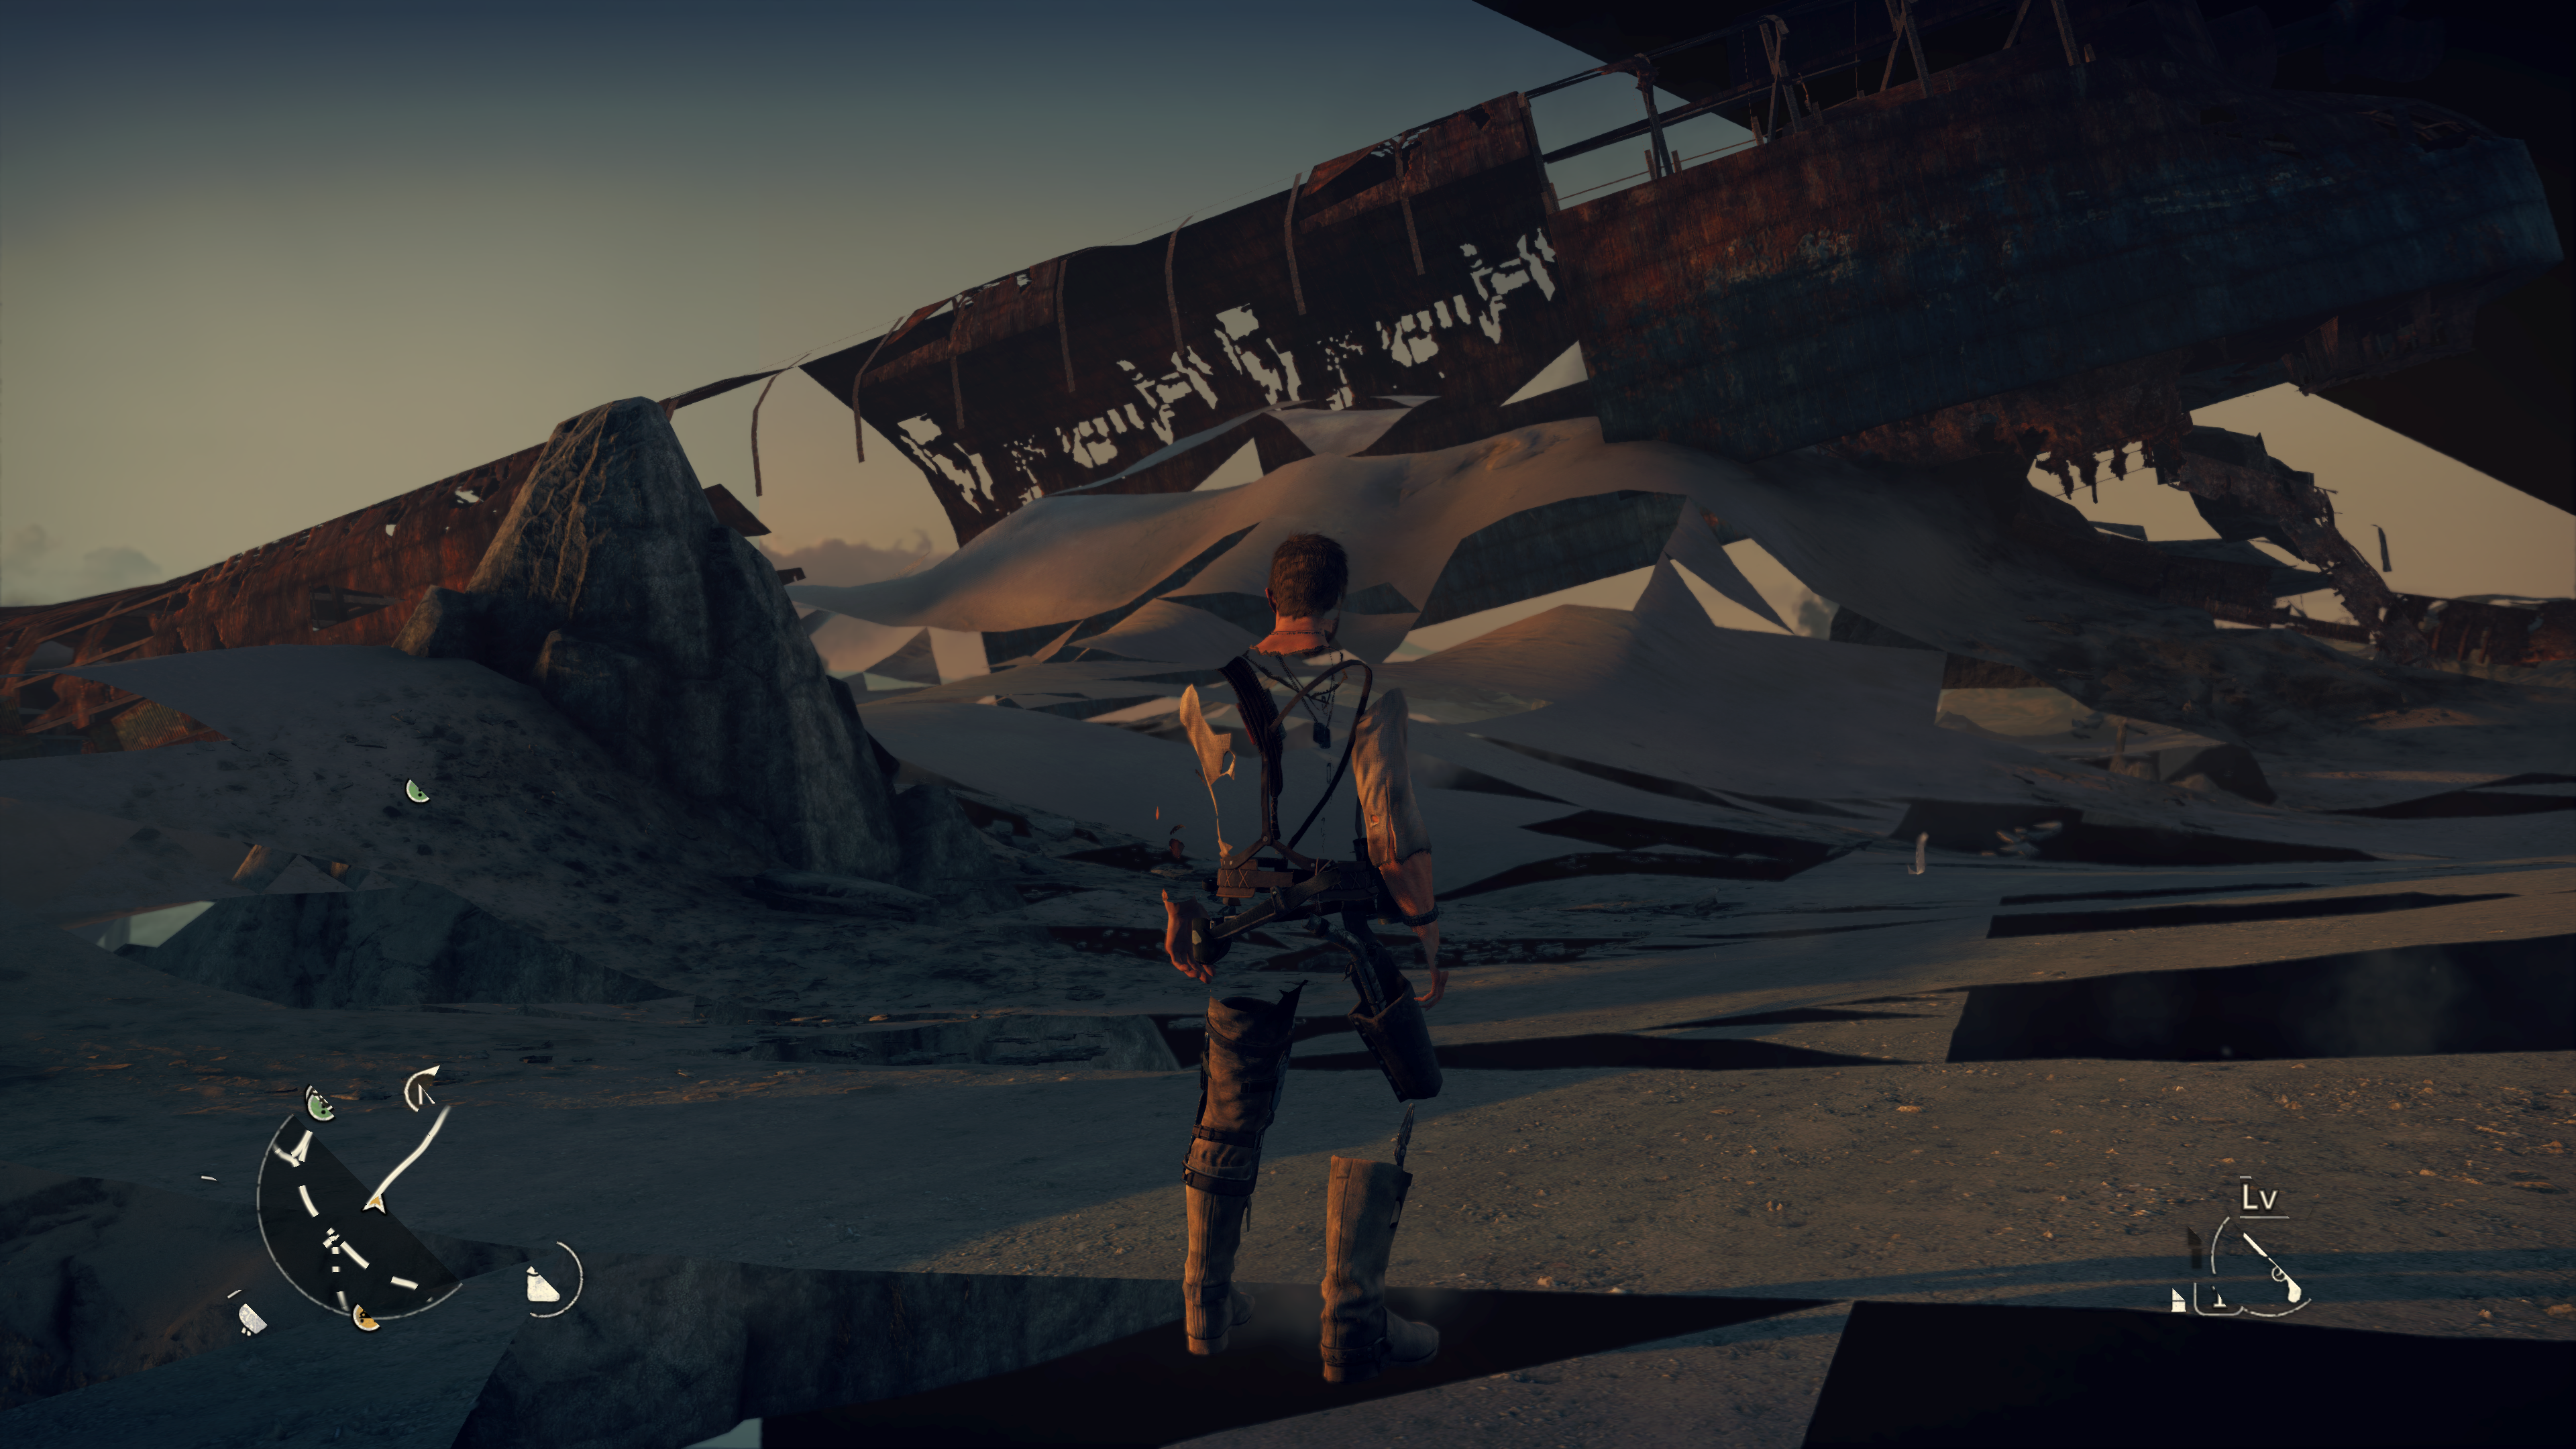
\includegraphics[scale=0.086]{images/hard1.png}
\includegraphics[scale=0.181]{images/hard2.png}
\vspace{5pt}
\caption[Examples of content-related artifacts]{Examples of content-related artifacts (images are courtesy of AMD).}
\label{fig:hard}
\end{figure}
\noindent
In order to manually reproduce different artifacts, we defined 13 classes of corruptions based on their appearance.
In the following sections, we will describe each artifact in detail.

\section*{Shader}
Shader is a program within GPU that governs frame rendering and determining various surface properties such as texture, reflection and lightning \cite{shader}. We define a class of corruptions---\textit{shader} artifacts, which are assumed to be caused by an incorrect operation of this program. Typically, shader artifacts are marked by the presence of polygonal shapes of a few different colors blended together or fading into transparency (see Figure \ref{shader}). This type of corruption was reproduced in Figure \ref{shader}.
\begin{figure}[H]
\centering
\includegraphics[scale=0.135]{images/shader1.png}
\includegraphics[scale=.42]{images/shader2.jpg}
\vspace{5pt}
\caption[shader artifacts]{shader corruption: actual (left) and reproduced with \texttt{Glitchify} (right).}
\label{shader}
\end{figure}
\section*{Shapes}
Unwanted random polygonal \textit{shapes} are also common in video games, especially in first-person shooting games. By inspection of the sample images, we conclude that shapes tend to appear in the darker part of the frame. The corrupted image provided by AMD shown in Figure \ref{fig:shapes} on the left exhibits thin black triangles that emanating from the center. To reproduce this artifact, \texttt{Glitchify} adds mono-colored polygonal shapes to the darkest region of the input image as shown on the right in Figure \ref{fig:shapes}.
\begin{figure}[H]
\centering
\includegraphics[scale=0.405]{images/shapes1.jpg}
\includegraphics[scale=0.43]{images/shapes2.jpg}
\vspace{5pt}
\caption[Shape artifacts]{shapes corruption: actual (left) and reproduced with \texttt{Glitchify} (right).}
\label{fig:shapes}
\end{figure}
\section*{Discoloration}
Another type of graphic artifact is \textit{discoloration}. As shown in the real corrupted image of Figure 2.4, the light spots of the image, which is a screenshot of game \textit{Civilization VI} become blue. The reason behind this phenomenon might be data overflow -- if we have an integer color value greater than 255, say 256, it will be cast back to 0. To produce a similar visual artifact, we randomly change the color of any pixel whose intensity exceeds a certain threshold. In our reproduced example image of Figure 2.4, the bright spots are painted white. We can choose the threshold to be based on the red, green or blue channel, or the overall intensity.

\begin{figure}[!ht]
\includegraphics[scale=0.132]{images/disco1.jpg}
\includegraphics[scale=0.152]{images/disco2.png}
\vspace{5pt}
\caption[Discoloration artifacts]{Discoloration artifacts: real corrupted image provided by AMD (left) and our reproduced corrupted image (right).}
\label{fig:discoloration}
\end{figure}

\section*{Random Patches}
The picture below on the left side illustrates the artifact of \textit{random patches}. In this particular image, the glitches are the small blue patches on the wall and the floor. The patches are usually part of an object, for example the wall. To reproduce this visual artifact, our program adds a random number of patches of random color and position to the image. We use segmentation algorithms \cite{watershed} to detect contours of objects so that the patches cover only part of a single object and do not lie on the edges of objects.

\begin{figure}[!ht]
\includegraphics[scale=0.128]{images/rp1.jpg}
\includegraphics[scale=0.16]{images/rp2.png}
\vspace{5pt}
\caption[Random patches artifacts]{Random patches artifacts: real corrupted image provided by AMD (left) and our reproduced corrupted image (right).}
\label{fig:rp}
\end{figure}

\section*{Dotted Lines}
In some corrupted images, we may also observe \textit{dotted lines}. For instance, in Figure 2.6 below, we can observe black dotted lines in the leftmost picture. This visual artifact is often hard to recognize unless we zoom-in on the corrupted picture. Our program includes two different methods to produce dotted-line artifacts. We either just add several dotted lines of random color and slope to the input frames, or we can have radial lines emanating from a single point.

%%%%%%%%
\newpage
%%%%%%%

\begin{figure}[!ht]
\includegraphics[scale=.35]{images/dl1.png}
\includegraphics[scale=.25]{images/dl2.png}
\includegraphics[scale=.45]{images/dl3.png}
\vspace{5pt}
\caption[Dotted line artifacts]{Dotted line artifacts: real corrupted image provided by AMD (leftmost), our reproduced corrupted image with random lines of green color (middle) and radial lines of red color (rightmost).}
\label{fig:dl}
\end{figure}


\section*{Parallel Lines}
In the screenshot of the League of Legends game (Figure \ref{fig:pl}), there are \textit{parallel lines} glitches. The color of the line segment is the pixel color of the starting point of the line. The method to generate parallel lines, clearly, is to add a random number of parallel lines whose colors are determined by the starting points.

\begin{figure}[!ht]
\includegraphics[scale=.2025]{images/pl1.jpg}
\includegraphics[scale=.135]{images/pl2.png}
\vspace{5pt}
\caption[Parallel line artifacts]{Parallel line artifacts: real corrupted image provided by AMD (left) and our reproduced corrupted image (right).}
\label{fig:pl}
\end{figure}


\section*{Square Patches}
Occasionally, gamers observe small \textit{square patches}, often with bright, blotches of color during gameplay. The square patches of the real glitched image provided by AMD (Figure 2.8) are purple or blue as highlighted in the red rectangle. To reproduce this glitch, we place some little square patches of random color on the input pictures. Our reproduced corrupted image on the right has cyan-blue square patches, highlighted in the red rectangle as well.
%%%%%%%%%%%%%%
\newpage
%%%%%%%%%%%%%

\begin{figure}[!ht]
\includegraphics[scale=0.64]{images/sp1.png}
\includegraphics[scale=0.32]{images/sp2.png}
\vspace{5pt}
\caption[Square patches artifacts]{Square patches artifacts: real corrupted image provided by AMD (left) and our reproduced corrupted image (right).}
\label{fig:sp}
\end{figure}



\section*{Texture Pop-in}
In computer graphics, textures are used extensively and are very important for rendering realistic 3-D images. \textit{Texture pop-in} refers to textures not loading in time or not loaded correctly. As a result, low-resolution textures appear instead of the high-resolution ones that gamers are expecting to see. To reproduce the texture pop-in artifact, we randomly select a region of the input image and then blur it by applying a Gaussian filter.

\begin{figure}[!ht]
\includegraphics[scale=0.32]{images/tp1.png}
\includegraphics[scale=0.425]{images/tp2.png}
\vspace{5pt}
\caption[Texture pop-in artifacts]{Texture pop-in artifacts: real corrupted image provided by AMD (left) and our reproduced corrupted image (right). The blurry regions due to texture-pop in are highlighted using red rectangles in both images.}
\label{fig:tp}
\end{figure}



\section*{Triangulation}
Some gamers have reported \textit{triangulation} artifacts \footnote{https://forums.warframe.com/topic/1095994-sanctuary-conduit-pixelated-screen-bug/}. These typically occur in intensive 3D games, where surfaces are rendered by numerous little triangles that form triangle meshes. Due to graphics defects, such triangular meshes are either displayed at a coarse resolution or displayed by sharp incorrectly colored triangles instead of smooth representations of surfaces. We developed two methods to reproduce this visual artifact. The first is regular triangulation, illustrated by the picture in the bottom left corner of Figure 2.10. To accomplish this, we randomly select a region which is then  divided into right triangles. The color of each triangle is determined by the weighted average of pixel colors within the triangle. The second is random triangulation, where we divide the regions into random triangles instead of right triangles using Delaunay triangulation\cite{delauny}.


\begin{figure}[!ht]
\includegraphics[scale=.152]{images/tri1.png}
\includegraphics[scale=.152]{images/tri2.png}\\
\includegraphics[scale=.13]{images/tri3.png}
\includegraphics[scale=.13]{images/tri4.png}
\vspace{5pt}
\caption[Triangulation artifacts]{Triangulation artifacts: real corrupted image found online (top row), our reproduced corrupted image with regular triangulation (bottom left) and random triangulation (bottom right).}
\label{fig:tri}
\end{figure}


\section*{Line Pixelation}
\textit{Line pixelation} is a peculiar type of gaming artifact that can have both subtle or pronounced effects. Through careful inspection of the left image in Figure \ref{fig:lp}, one can spot the line pixelation artifact at the very bottom of the picture. In order to capture the distribution (pixel intensity variations) in this kind of artifact, we inserted a random number of noisy stripes with random orientations and positions.

\begin{figure}[!ht]
\includegraphics[scale=0.143]{images/lp2.png}
\includegraphics[scale=.836]{images/lp1.png}
\vspace{5pt}
\caption[Line pixelation artifacts]{Line pixelation artifacts: real corrupted image provided by AMD (left) and our reproduced corrupted image (right).}
\label{fig:lp}
\end{figure}


\section*{Screen Stuttering}
Screen \textit{stuttering} was one of the most interest artifacts to figure out. The image on the top left of Figure \ref{fig:stuttering} is the corrupted image we received from AMD. We first had to figure out what the normal image looked like before we could reproduce this artifact. The image on the top right shows what one of our team members cleverly did to figure out the normal image. We discovered that screen stuttering occurs when neighboring columns and rows of the image are swapped. In this way we were able to recover the original image (bottom left), and then reproduce this artifact (bottom right).

\begin{figure}[!ht]
\centering
\includegraphics[scale=0.29]{images/stutter1.png}
\includegraphics[scale=0.458]{images/stutter2.png}
\includegraphics[scale=0.68]{images/stutter.png}
\includegraphics[scale=0.11]{images/stutter3.jpg}
\vspace{5pt}
\caption[Screen stuttering artifacts]{Screen stuttering artifacts: real corrupted image provided by AMD (top left) and our reproduced corrupted image (bottom right).}
\label{fig:stuttering}
\end{figure}

\section*{Screen Tearing}
One of the most common gaming artifacts is \textit{screen tearing}. Screen tearing occurs when two consecutive frames in a video get rendered into the same image. Therefore, part of the image shows the scene at a certain point in time, while the other part of the same image shows that scene at a later time. In order to reproduce this type of artifact, we select two frames in a video that are 100 frames apart from each other, and then randomly replace some rows (or columns) of the first frame with the corresponding rows (or columns) of the second frame. Examples are shown in Figure \ref{fig:tearing}.

%%%%%%%%%%%%%%%%%%
%%%%%%%%%%%%%%%%%%
\newpage
%%%%%%%%%%%%%%%%%%
%%%%%%%%%%%%%%%%%%

\begin{figure}[!h]
\includegraphics[scale=0.29735]{images/tearing1.jpg}
\includegraphics[scale=0.627]{images/tearing2.png}
\vspace{5pt}
\caption[Screen tearing artifacts]{Screen tearing artifacts: real corrupted image provided by AMD (left) and our reproduced corrupted image (right).}
\label{fig:tearing}
\end{figure}


\section*{Morse Code Pattern}

\textit{Morse code} pattern (shown in Figure \ref{fig:morse}) appears when memory cells on a graphic card become stuck and display their stuck values on the screen rather than displaying the true image. Over-clocking and over-heating are two possible causes of such memory corruption. Over-clocking refers to the action of running a GPU at a higher speed than it is designed to run, and over-heating refers to running a GPU such that its temperature exceeds its maximum specified operating temperature. In order to reproduce this type of artifact, we add morse-code-like patterns to random locations in the frame, as shown in Figure \ref{fig:morse}.

\begin{figure}[!h]
\includegraphics[scale=0.765]{images/morse1.png}
\includegraphics[scale=0.288]{images/morse2.png}
\vspace{5pt}
\caption[Morse code artifacts]{Morse code artifacts: real corrupted image extracted from online YouTube video (left) and our reproduced corrupted image (right).}
\label{fig:morse}
\end{figure}


\section*{Glitchify Software}
% \textcolor{red}{Add the software interface here}. \textcolor{red}{You don't have to discuss all the options, but give a few examples. Also use the textt font to show code.}

\noindent In order to generate a large number of corrupted images, we implemented a software named ``Glitchify" that takes in images and videos and outputs corrupted images. The software interface is shown in Table \ref{interface}.
\begin{center}
\begin{table}
\scalebox{0.87}{
\begin{tabular}{ |c|c| } 
 \hline
 Input Argument & Description \\ 
  \hline
 "Input" & Path to the directory that contains input images and/or videos. \\ 
  \hline
 "Output" & Path to the directory where output images are saved. \\ 
 \hline
  "Artifact Type" & Type of artifact to be inserted to the input images/videos.\\ 
   \hline
   "Interval" & Number of frames skipped before the next frame where artifacts are inserted.\\
   \hline
   "Output Array" & Whether to output the corrupted images in the format of numpy array.\\
      \hline
      "Resize Output" & Whether to resize the corrupted images to a specified size.\\
    \hline
\end{tabular}}
\caption{\label{interface}Interface of the \textit{Glitchify} software.}
\end{table}
\end{center}
\subsection*{Generating Training, Testing, and Holdout datasets}

\noindent We used the newly created \texttt{Glitchify} program to generate these artifacts and obtained a large dataset. \\


\noindent In order to achieve this, we downloaded long (2-6 hour) gameplays of different video games. We then extracted around 2,000 images from each game until we had a total of 50,000 images. We manually scanned the extracted frames to ensure that they are not already corrupted to the best of our abilities. This was a cumbersome and error prone process as we had to make (subjective) decisions as to whether the features we were seeing in some frames were part of the gameplay experience or not. For example, the two images illustrated in Figure \ref{fig:hard} are examples of frames where it is not clear whether they are corrupted or normal. We made an effort to exclude all the images that were ambiguous from our data set. After extracting normal images, we then created a uniform distribution of different kinds of artifacts with half of the images, leaving the other half intact as ``normal" images. \\

\begin{figure}
\centering
\includegraphics[scale=0.11]{images/line_pixelation_39.png}
\includegraphics[scale=0.11]{images/line_pixelation_68.png}
\caption{Examples of frames that are hard to label}
\label{hard}
\end{figure}


\noindent Since we extracted high-quality images (1920 pixels x 1080 pixels x 3 color channels), the dimensions of the images were too large to be used by our models. We often experienced unexpected memory error when we loaded the images in our programs, and we did not have enough RAM to feed the original sized images into our models. Additionally, nearby pixels in images are often related, therefore by feeding an entire image into a model we are giving it a lot of repetitive information. Our solution to this problem was to use various feature representations of the images, whose dimensions are much smaller than those of the original images. In the next chapter we will discuss the features that we considered.

\begin{table}[h]
\centering
\includegraphics[scale=0.8]{tables/games.pdf}
\caption{Games from which the images were extracted.}
\label{games}
\end{table}


\endinput
